\documentclass[12pt,a4 paper,title page]{article}
% \documentclass{article}
\usepackage[utf8]{inputenc}
\usepackage{microtype}
\usepackage[british]{datetime2} % For urldate formatting
\usepackage{natbib}
\usepackage{graphicx}
\usepackage{float}
\usepackage{textcomp}
\usepackage{xcolor}
\usepackage{soul,color}
\usepackage{amsthm}
\usepackage{bm}
\usepackage{algorithm}
\usepackage{algorithmic}
\usepackage{amsmath,amssymb,amsfonts}

\theoremstyle{definition}
\newtheorem{definition}{Definition}[section]
% \renewcommand{\algorithmicrequire}{ \textbf{Input:}} %Use Input in the format of Algorithm  
% \renewcommand{\algorithmicensure}{ \textbf{Output:}} %UseOutput in the format of Algorithm 

\usepackage[colorlinks = true,
            linkcolor = teal,
            urlcolor  = teal,
            citecolor = blue,
            anchorcolor = blue]{hyperref}
\usepackage{wrapfig}



\bibliographystyle{uts} % Import Harvard UTS style
\setcitestyle{aysep={}} % Remove comma separation between author and year for in-text citations
\title{Research Proposal: Heterogeneous Information Network based Recommender System}
\author{\large\textbf{Di Zhang}, \\
\textbf{supervisor: Professor Guanquan Zhang}, \\
\textbf{co-supervisor: Professor Jie Lu}, \\
\textbf{Student number: 31292711}}

\date{\Large{\textbf{October 2019}}}

\begin{document}
\sloppy
\maketitle
\hfill
\hfill

\section*{Summary}

\subsection*{Topic} Heterogeneous Information Network based Recommender System

\subsection*{Keywords} 

Recommender system, Heterogeneous Information Network, Knowledge Graph, Data Mining 

\subsection*{Thesis statement 1}
The Embedding based feature mining in Heterogeneous Information Graph would both reduce recommendation system implementation complexity and enables model to be adaptive to new information over time

\subsection*{Thesis statement 2}
By learning semantic information of Heterogeneous Information Network via its nodes and edgers can help in developing a generic embedding approach for implementing real-world recommender systems that is long lasting and easy on maintenance. 

\subsection*{Aim 1}
To explore the semantic information relationship within Heterogeneous Information Network for Recommendation problem.

\subsection*{Aim 2}
To understand the effectiveness and adaptability of Heterogeneous Information Network for constant data stream processing in recommendation problem domain. 

\subsection*{Aim 3}
Try to develop a generic approach based Heterogeneous Information Network to make a long-lasting recommender system that is both adaptive to feature changes and being temporal aware. 

\subsection*{Objective 1}
To develop a formalized graph structure modelling methodology for rich feature data sets. 

\textbf{Success condition:} Load raw data set into a graph structure that can effective present the information required for recommendation problem accordingly 

\subsection*{Objective 2} 
To develop a comprehensive similarity method based on graph structure that can applied into recommender systems. 

\textbf{Success condition:} Evaluate current graph-based similarity measures to determine and develop a fitting similarity approach for recommender system, which is, capable of solving Top-K recommendation and effective in Cold Start problems. 

\subsection*{Objective 3}
To develop a semi-supervised feature mining method to handle complex large heterogeneous information network. 

\textbf{Success condition:} An embedding approach that is not only performant but also computational effective for mining large scale HIN. 

\subsection*{Objective 4} 
To develop a graph-based learning framework that adaptive to tempo information 

\textbf{Success condition:} A graph-based framework that is capable learning feature changes over time. 

\subsection*{Objective 5} 
To develop a recommendation system based on Heterogeneous Information Network 

\textbf{Success condition:} A working recommender framework prototype using generic approach that is capable to  adapting to feature change and computational effective.  

\newpage

\section{Introduction and background}
Recommender System (RS) is an indispensable technology in this big data era. It evolves around our everyday life on multiple fronts. From daily curated news feed, to online shopping portal, to music playlist that we listen, and movies we watch. RS help us to find personalized interests from the ever-increasing information overloads \citep{Lu2015}. It is also acting as a decision-making assisting agent, that makes peoples life more efficient and focused. 

\subsection{Research landscape}

2006, 100 million datasets were released by Netflix \citep{Bennett2007} The action expedited the research on Collaborative Filtering. Over decades, Collaborative Filtering is still at the forefront of Recommender systems Field. Many new approaches and extensions had been developed in collaboration with Collaborative Filtering to tackle its cold start and data sparsity problems. \citet{barkan2016item2vec} introduced item2vec for Collaborative Filtering also showed how different forms of recommendations can be used within Collaborative Filtering domain. 

On the deep-learning camp, recommender system is also striving by utilizing the learning ability of Neural Network. \citet{Cheng2016} proposed `Wide and deep learning for recommendation system` to achieve both memorization and generalization in recommendation for Google Play. \citet{Covington2016} demonstrated how deep neural network is implemented in YouTube, which helped billions of users discover their personalized content. \citet{Karatzoglou2013} proposed use Reinforcement Learning techniques personalized ranking based on users’ interests.  

Transfer Learning \citep{Pan2010} in Cross Domain recommender system is another promising area which make recommendation possible in when initial user interaction data is scarce in target domains. \citet{Elkahky2015} experimented this approach on multiple Microsoft products, and concluded multi domain recommendation system significantly outperforms single domain recommendation systems. 

\subsection{Industry Challenge}

However, a good working recommendation system is not just about recommendation algorithm, it is a systematic approach. Being overwhelmingly popular, Collaborative Filtering success is not only due to its effectiveness, but also thanks to its simplicity in data engineering requirement and domain knowledge dependency \citep{Amatriain2016}. CF is one of the most accessible recommendation approaches for a lot of recommendation solutions, despite of having known issue with data sparsity and cold start problems.

Based on observation, the challenges of setting up a successful real-world recommender system mainly comes down to 3 parts:  

\begin{itemize}
\item Algorithm. Setting up an effective recommendation system is different for every business and every problem. A algorithm in recommender system is very hard to kept generic. Thus, transferability and reusability is low.

\item Data Adaptation. In the real-world scenario, information in flow as data streams. Features changes as time go by, along with recommendation objective. We often see diminishing performance from a developed recommender system over time. The ability to adapt data dynamics and making use of Temporal Information remain challenging in recommendation field.

\item Data Mining. Researcher and developers normally facing enormous yet complex datasets, in which, only small percentage can be effectively utilized for recommendation learning. In many instances, big data brings not only valuable features information for learning tasks, but also, inevitably introducing noises alone the way. In place a computational effective data mining methodology is a key building block for recommender system.
 
\end{itemize}

Living in a world of information, the information objects or data points around us are mostly interconnected with each other as a complicated network. Heterogenous Network, in a lot of time can serve as a reflection of real-world information without loss of generality. World wide web, biology networks, as well as traffic system, etc. can all be formed into an information network. Based on existing research, Heterogeneous Information Network had shown a lot of promises in the data mine field. Several of promising research progress has had been achieved in the HIN space. 

Known for its Semitic properties, Heterogeneous Information Network captures information and relationship between different types of data points. Comparing with traditional column-based data structure, Its adaptability in every changing data context, is much more forgiving for dynamic data models. Nodes and Meta-Path information mining is playing an important role in the data mining research domain. In recommender systems, a lot of time, we are tasked to making recommendations based on similarity. Techniques such PathSim \citep{Sun2011PathSim} and HeteSim \citep{Shi2013HeteSim} provided a rich foundation for similarity measure in HIN. Its results can be naturally borrowed into recommender system in KNN settings and Top-K recommendations. 

In the feature learning space, node2vec (Grover and Leskovec 2016), an algorithmic framework for learning continuous feature representations for nodes in networks. In node2vec, nodes is mapped to low-dimensional space of features that maximizes the likelihood of preserving network neighborhoods of nodes. Using a biased random walk procedure to explores diverse neighborhoods, node2vec can learn task-independent representations in complex networks. GraphSAGE (Hamilton et al. 2018) furthered the graph feature learning to be inductive instead of requiring all nodes in the graph to be presented during training of the embeddings. This extend the graph generalization ability to unseen nodes. From recommender system perspective, allowed less dependency of background knowledge in the recommendation problem domain \citep{Hu2018}.  

Graph Classification using Structural Attention \citep{lee2018graph} is a good demonstration of attention-based learning techniques are applied in graph. Such feature learning ability makes a graph based data feature to be more versatile in facing data change and problem context switching. 
Techniques, such as, User-guided embedding, can be invaluable for catering to recommender system with ever changing data streams. Such approach can also effectively reduce the data noise problem by exploiting the signals residing in the data.  

Graph Neural Network (GNN) as an extension of deep learning approaches using graph data network structure have recently emerged. \citet{ying2018graph} shows promising signs of GNN being adopted in a large-scale deep recommendation engine. \citet{song2019session} propose a recommender system that model dynamic user behaviors and context-dependent social influence with a graph-attention neural network, which dynamically infers the influencers based on users’ current interests. Both of the research shown that GNN would be a promising approach for handling dynamic and temporal data in recommendation tasks.

\section{Aims}
\subsection{Aim 1}
To explore the semantic information relationship within Heterogeneous Information Network for Recommendation problem.

\subsection{Aim 2}
To understand the effectiveness and adaptability of Heterogeneous Information Network for constant data stream processing in recommendation problem domain. 

\subsection{Aim 3}
Try to develop a generic approach based Heterogeneous Information Network to make a long-lasting recommender system that is both adaptive to feature changes and being temporal aware. 

\section{Objectives}
This research aim to achieve following objectives: 

\subsection{To develop a formalized graph structure modelling methodology for rich feature data sets.  }

Develop a generic approach to project users, items, and their related feature information into a holistic heterogeneous Information Network. For Recommender System, HIN will not only need to handle handle complex structures. So that, both user-item interaction, commonly being used for collaborative filtering approach. User Profile, Item Attribute, which widely adopted in content based recommender system, can be fused in to single Multiple-Hub Network \citep{Shi2017} structure.

\subsection{To develop a comprehensive similarity method based on graph structure that can applied into recommender systems. } 

For the heterogenous information graph, evaluate the similarity of objects is the fundamental in data mining. In recommender system, it faces ever growing and evolving dataset. Working against massive datasets, and complex data transformation are common obstacles for producing a high quality recommendation solution. Developing an computational efficient similarity measure that fits for recommender system's use case, is a key milestone to ensure my research success.

\subsection{To develop a semi-supervised feature mining method to handle complex large heterogeneous information network.}

The rich information contained within the same HIN may only useful for certain recommendation problems. Nodes and path would have different weights when optimization objective or time is different. Developing a semi-supervised mining method would help recommender system to find different weights on based on the inter relationship between nodes and meta-paths. Reducing complex features into lower dimensions would also helping reduce the computation complex \citep{Cai2018} as mentioned in Object 2, Further simplify implementation difficulties in recommender systems. 

\subsection{To develop a graph-based learning framework that adaptive to tempo information}

Time factor is an important factor for making recommendations. Users past context could have direct impact of user current interest. \citet{Song2019} had shown that measurable improvement performance can be found in recommender system, when exploiting time information in the recommendation process. As a extension objective from Objective 2 and 3, including temporal dynamics and considering the transitive similarity between nodes and edges is another important factor in delivering quality results.

\subsection{To develop a recommendation framework based on Heterogeneous Information Network} 

By putting research results from Objective 1,2,3 into a holistic framework, would enable us to develop a generic approach and making recommendation model adapting changes could significantly reduce the recommendation systems maintenance cost and keeping system performance over time. 
Instead of focusing the recommendation research on static datasets. In this research, we are trying to solve the real-world recommendation problem in a dynamic angle.

\subsection{To develop a recommender system case study for validating the proposed approaches}

Following common datasets will be used for method verification: 

\begin{itemize}

\item MovieLens dataset (http://grouplens.org/datasets/movielens/) 

\item Netflix dataset (http://www.lifecrunch.biz/archives/207) 

\item DBLP Citation Networks (https://dblp.uni-trier.de)  

\end{itemize}

Case studies on real estate and tourism recommendation will be conducted to validate the user-interest drifts overtime, to show how graph-based approach adapts to the ever-evolving data changes. 

\section{Methodology}

\subsection{Task 1: propose a graph structure modeling methodology for recommender system}
It is challenging to develop effective data extraction and exploitation methods for Heterogeneous Information Network based recommender system.

\subsubsection*{Step 1: develop a generic graph structured data for recommendation problem}

Graph structure is being adopted in a wide range of applications. However, to our best of knowledge, none of them is taking a generic approach in forming the heterogeneous graph for recommender systems. HIN normally only optimized for a specific problem, and less adaptable to information evolution over time. 
Based on the nature of recommender system, we propose to accommodate not only user-item interaction, item features, and user profile information into the same heterogeneous information network. We also propose to further explore the semantic information by normalizing features on both item feature and user profile information into more atomic feature nodes. such practice would bring multiple benefits: 

\begin{itemize}
    
\item[1] Reduce data sparsity. By breaking up item features into more generic feature nodes would help increase the density of the network, and increase possible connectivity (mate-path) between nodes.

\item[2] With that, new in coming information would also transformed through the same decomposing process, hence making the graph structure adaptable to ever evolving changes.

\item[3] As the information graph cumulates auxiliary information in a holistic approach, suc structure also making problem context switch possible.

\end{itemize}

Of course, having a generic purpose HIN as training source introduce both complexity and noise. which we would discuss in Task 2 and Task 3.


\subsubsection*{Step 2: to develop transformation rule for the graph structure}

Recommendation test data sets are normally saved in csv format, which is quite different from the graph data structure we proposed above. Multi-Hub Network structure will be developed to transform the flat user-item data sets into a holistic feature-rich graph structure. Fig. \ref{fig:multihub}

\begin{figure*}[!t]
    \centering
    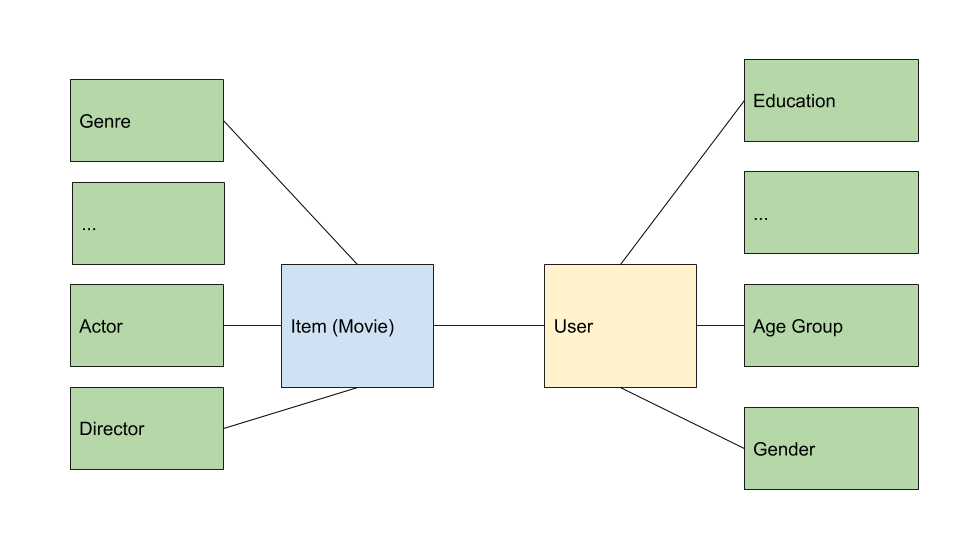
\includegraphics[width=0.8\textwidth]{figs/multi-hub.png}
    \caption{a multi-hub network structure based on Movielens data}\label{fig:multihub}
\end{figure*}


\subsection{Task 2: develop a comprehensive graph similarity measure}

Similarity measure the basis of many recommendation tasks, It evaluate the proximity among objects. Feature-based and link-based approaches are 2 main Similarity measures in HIN. 

The feature based approaches measure the similarity of objects based on their feature values, such as cosine similarity, Jaccard coefficient, and Euclidean distance. The link based approaches measure the similarity of objects based on their link structures in a graph. 

Similarity measure on HIN not only considers structure similarity of two objects but also takes the meta-path between two objects into account \citep{Shi2017}. \citet{Sun2011PathSim} propose PathSim that measure the semantics structure in meta-paths constituted by different-typed objects. The intuition for a single Meta-Path measure can be seen as: if source entity and target entity are exactly the same, then the round trip Meta-Paths $\mathcal{P}_1: A_1 \xrightarrow{r_1} A_2$ and 
$\mathcal{P}_1^{-1}: A_2 \xrightarrow{r_1^{-1}} A_1$ are always symmetric.

\theoremstyle{definition}
\begin{definition}[PathSim \cite{Sun2011PathSim}]\label{def:pathsim}
    Given a Meta-Path $\mathcal{P}$, PathSim between two entities $x$ and $y$ is:
    \begin{equation}
        sim(x,y)=\frac{2 \times \{|p_\text{x...y}:p_\text{y...x}| \in P\}}{\{|p_\text{x...x}:p_\text{x...x}| \in P\} + \{|p_\text{y...y}:p_\text{y...y}| \in P\}}
    \end{equation}
    where $x$ stands for source node, while $y$ for target node. 
    $x, y$ shares the same entity type $A_i$.
    $p_\text{x...y}$ stands for Meta-Path between entity $x$ and $y$. 
\end{definition}

HeteSim \citep{Shi2013HeteSim} proposed evaluate the relevance of any object pair under arbitrary meta-path. \citet{xiao2016avgsim} further improved HeteSim computation efficienc with AvgSim on large scale data.

For recommender systems, its a common use case for item-item and user-item recommendations based on similarity. Those measure is especially valuable when user-item interaction data is scarce, such as cold start problem. 

\subsection{Task 3: use embedding approach of large scale Information Network}

In recommendation settings, if we consider the graph structured HIN as a generic data repository. Such repository is not only capable of capture inter-relationship and semantic information between different types of data points (nodes). it is also adaptive to new information and grow the network organically. This allows HIN data repository capable contain rich information for complex recommendation problems. The challenge comes with a ever growing a graph network, is the noises increase alone with information cumulation.

Effective graph analytics provides users a deeper understanding of what is behind the data, and thus can benefit a lot of useful applications \citep{Cai2018}. Graph embedding is an effective yet efficient way to solve the graph analytics problem, while reduce the high computation and space cost, where the network structural information and graph properties are preserved into a low dimensional space.

Apart of overcoming computation constrains, embedding also play a important role of distilling relevant information, reducing noises for accordingly recommendation problem.

In order to learn effective heterogeneous network representations for summarizing important structural characteristics and properties of HINs. Based off work of DeepWalk \citep{perozzi2014deepwalk} and Node2Vec \citep{grover2016node2vec}, we characterize nodes from HINs with low-dimensional vectors, i.e., embeddings. 
Compared with meta-path based similarity, instead of relying on explicit path connection, embedding encode valuable feature data with latent vectors. The learned embeddings are in a more compact form that is easy to use and integrate. 
Motif-based approach \citep{tsourakakis2017scalable} and attention based approach \citep{Hu2018}, \citep{lee2018graph} yield effective results in both data mining and recommendation research filed.
Last but not least, embedding approach creates denser data, that make the recommender system being more resistant to noisy and sparse data. 

Followed by Task 2 similarity measure. In recommender system, we normally consider nodes proximity base on the weights of connecting edge between source and target nodes. As illustrated in GraRep \citep{cao2015grarep}. The model learns low dimensional vectors to represent vertices by integrates global structural information of the graph into the learning process.

On the other hand, GraphSAGE defined nodes proximity by comparing nodes' neighborhood. It introduced a general inductive framework to efficiently generate node embeddings for previously unseen data by leveraging node feature information. \citet{hamilton2017inductive} uses function that generates embeddings by sampling and aggregating features from a node’s local neighborhood.

Subsequently, fusion functions is used to integrate multiple node or meta-path embeddings into a single representation for recommendation. These fusion functions provide flexible ways to transform HIN embeddings into useful information for recommendation.


\subsection{Task 4: extend Heterogeneous Information Network to accommodate temporary information through time}

Most of the research mentioned above is based on static data. After defining suitable Similarity Measure (Task 2) and fitting Embedding Approach (Task 3) for the recommender system. In this task we would like to extend previous tasks to include temporal information, and data dynamics for our recommender system to taking account. \citet{he2014exploiting} extend the meta
path-based similarity measure PathSim by incorporating richer information, such as
transitive similarity and temporal dynamics. 

At the same time, in order to make HIN based recommender system to be time aware. Architecture adjustment is required accordingly. Graph Spatial-temporal Networks aim to learn unseen patterns from spatial-temporal graphs, which are increasingly important in many applications \citep{wu2019comprehensive}. 
The goal of graph spatial-temporal networks can be forecasting future node values or labels, or predicting spatial-temporal graph labels. Recent studies have explored the use of GCNs for action recognition \citep{yan2018spatial}, and GCNs in combination of with RNN \citep{li2017diffusion} or CNN \citep{yu2017spatio} in transportation traffic prediction.

So far GCNBased Graph Spatial-Temporal Networks have limited implementation in the recommender system. Based on the embedding methodology mentioned in Task 3, users and item nodes relationship can be treated as adjacency matrix, hence, user can be represented as a summation of K adjacency matrices of item-user edge. Subsequently, Graph Convolution can then applying different weights to its neighboring edges and sum them. By extending the temporal flow as graph edges, using a unified GCN model, spatial and temporal information can be extracted jointly.

\subsection{Task 5: develop recommendation framework based Heterogeneous Information Network}

Due to the flexibility in modelling data heterogeneity, HIN based recommendation adopts the model complex characterize and heterogeneous auxiliary data for recommender systems.

\subsubsection*{Step 1: HIN based recommendation on static data sets}
There are mainly 2 approaches in static data settings for performing recommendation tasks via HIN. 

Similarity base approach, which is mostly mentioned in task 2. The strength of similarity based approach are mostly comes down to computation efficiency. some of the approaches, such as PathSim \citep{Sun2011PathSim}, and AvgSim \citep{xiao2016avgsim} had been well researched and have a number mathematical optimization for recommender problem. however, latent structure features of users and items relationship are not fully used, when using path/node based similarity methods.

Alternatively, as mentioned in task 3, node embedding and meta-path embedding had been a rising research topic in recently years. Notables, \citet{shi2018heterogeneous} had proposed using node embeddings are first transformed by a set of fusion functions, and then extend the information into a matrix factorization (MF) model. The extended MF model together with fusion functions are jointly optimized for the rating prediction task.

\subsubsection*{Step 2: HIN based recommendation on dynamic temporal data sets}

In real-world settings, users interest is dynamic and influenced by the past experience. Temporal information is important for improving recommendations' accuracy. However due to the complexity of graph structure and computation restrictions. its a big challenge for reflecting both information into recommender system. Recent development in Graph Neural Network (GNN) and Attention Model had shown some exciting development in taking account of temporal information and user-item interaction sequences \citep{yu2017spatio}.  

There are two basic approaches currently exploring how to generalize CNNs to structured data forms: 
The First is to expand the spatial definition of a convolution \citep{niepert2016learning}. It rearranges the vertices into certain grid forms to perform convolution operations. The Second is to manipulate in the spectral domain with graph Fourier transforms \citep{bruna2013spectral}. Spectral graph convolution uses spectral framework to apply convolutions in spectral domains.

\citet{song2019session} propose a dynamic-graph-attention neural network based recommender system for online communities. \citet{Hu2018recommender} propose a unified model LGRec to fuse local and global information for top-N recommendation in HIN.


\subsection{Task 6:  A case study for validating the proposed recommendation approaches}

The research will be verified from two aspects: 

First, public datasets, such as DBLP DBLP Citation Networks, MovieLens data sets (http://www.grouplens.org/node/73), will be used to verify the effectiveness of the graph modeling approach for recommender system. Similarity measure as well as adaptability are the core parts of the approach, each aspects will be verified accordingly. 

Second, the approach will be used in a real world data sets. Real data sets from the tourism and real-estate industry will be used to further test the effectiveness of the method.




\section{Future Impact/Significance}

\subsection{Practical Significance Analysis}
Recommender system is becoming more and more prominent in people's daily time. Users are overwhelmed by information that is pushed by different entities. Identify users' interest to assists decision making is an important mission for recommender systems. Meanwhile, due to the nature difference among different industry and business, implementing and productionize a recommender system into real-world use, normally require big effort. An effective recommender system often heavily relied on domain knowledge and tailor-made solutions. What's more, most of the existing recommender system needs constant maintenance and adjustment.  

Collaborative Filtering based recommender system gains a lot of traction in the industry. To my view, that is not only because the model can perform under certain conditions, its popularity is also gained due to its engineering simplicity and being a generic to different kinds of industry and business background. Heterogeneous Information Network based recommender system persists information objects with semantic network structures. It allows new information to be adapted and reflected relatively easy by extending relationship between new information objects (nodes, edges).  

Thus, developing a generic HIN approach for recommender system could significantly simply engineering complexity and “bring to live” cost for business to be benefiting from having recommender system in place. 

\subsection{Theoretical Significance Analysis}
Research on Recommender System seldomly considers feature adaptability along with temporal information progression. Most of the recommender system research treats recommendation problem as a static snapshot of time. The consequences of such approach means the subtle change between time period is not being used for making recommendations. This also makes the assumptions that datasets would not change significantly over time, such as new important features would not merge in future period, even though constant change is a key characterize of real-world datasets. 

For this study, we are focusing adaptability for recommender systems by leverage HIN network structure.  In this way, this research will improve recommender systems ability in accommodating changes. 

The result will help making a long-lasting effective recommender system, while reduce the maintenance cost of recommendation models. 

\clearpage

\bibliography{bibliography}

\end{document}
